\documentclass{article}

\usepackage{graphicx}
\usepackage{lmodern}
\usepackage[T1]{fontenc}
\usepackage{amsmath}
\usepackage{correctmathalign}

\title{Correction Spacings: eqnarray(*), aligned, alignedat, and gathered}
\author{Yuwsuke Kieda}
\date{2017/04/04 v1.1}

\renewcommand\labelitemi{\textendash}

\begin{document}
\maketitle

\section{Descriptions}

We will realignment some expression environments spacing.
It is a correction in the horizontal spacing of the alignment.

\section{Usage}

\subsection{Preamble}

\begin{verbatim}
\usepackage{amsmath}
\usepackage{correctmathalign}
\end{verbatim}

Remark: amsmath package is optional: if you use aligned, alignedat, or gathered environments.

Remark: The problem with the amsmath package (2016/11/05 2.16a) was solved by the original. See the options \texttt{alignedleftspaceyes}, \texttt{alignedleftspaceno}, and \texttt{alignedleftspaceyesifneg}.
We dealt with versions prior to 2016/03/10 v2.15b.

\subsection{Options}

\begin{itemize}
 \item \verb!latexorg!: original behavior of LaTeX/amsmath package
 \item \verb!fleqn!: corresponds to class file and/or amsmath package's fleqn option
\end{itemize}

\section{File with Original Definitions}

\begin{itemize}
 \item \verb!eqnarray!: latex.ltx
 \item \verb!\start@aligned! and \verb!\gathered!: amsmath.sty (before 2016/03/10 v2.15b)
\end{itemize}

\section{License}

BSD 2-Clause License

\section{Samples}

Cf.\ defaults of \LaTeX{}\ and \texttt{amsmath.sty} before 2016/03/10 v2.15b (Figures~\ref{fig1} and~\ref{fig2}).

\setbox9\hbox{Figure 1: \texttt{eqnarray*} environment}%
\setbox8\hbox{Figure 2: \texttt{aligned} environment}%
\begin{figure}
 \centering
 \begin{minipage}[t]{\wd9}
  \centering
  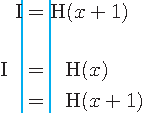
\includegraphics{eqnarray-org.pdf}
  \caption{\texttt{eqnarray*} environment by \LaTeX{}\ default.}
  \label{fig1}
 \end{minipage}\qquad
 \begin{minipage}[t]{\wd8}
  \centering
  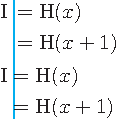
\includegraphics{aligned-org.pdf}
  \caption{\texttt{aligned} environment by \texttt{amsmath.sty} default (before 2016/03/10 v2.15b).}
  \label{fig2}
 \end{minipage}
\end{figure}

\noindent
\begin{center}
 \makeatletter\@wholewidth0pt\makeatother
 \frame{%
 \begin{minipage}{\wd9}
  \[
  \mathrm{I} = \mathrm{H}(x + 1)
  \]
  \begin{eqnarray*}
   \mathrm{I} &=& \mathrm{H}(x)\\
   &=& \mathrm{H}(x + 1)
  \end{eqnarray*}
 \end{minipage}}\qquad
 \frame{%
 \begin{minipage}{\wd8}
  \begin{align*}
   \mathrm{I} & \begin{aligned}[t]
                 &= \mathrm{H}(x)\\
                 &= \mathrm{H}(x + 1)
                \end{aligned}\\
   \mathrm{I} &= \mathrm{H}(x)\\
   &= \mathrm{H}(x + 1)
  \end{align*}
 \end{minipage}}
\end{center}


\subsection{Use \LaTeX{}\ code}

\begin{verbatim}
\[
 \mathrm{I} = \mathrm{H}(x + 1)
\]
\begin{eqnarray*}
 \mathrm{I} &=& \mathrm{H}(x)\\
            &=& \mathrm{H}(x + 1)
\end{eqnarray*}

\begin{align*}
 \mathrm{I} & \begin{aligned}[t]
               &= \mathrm{H}(x)\\
               &= \mathrm{H}(x + 1)
              \end{aligned}\\
 \mathrm{I} &= \mathrm{H}(x)\\
            &= \mathrm{H}(x + 1)
\end{align*}
\end{verbatim}

\end{document}